\documentclass[12pt,a4paper]{article}

% ── Packages ──
\usepackage[margin=2.5cm, headheight=14pt]{geometry}
\usepackage[utf8]{inputenc}
\usepackage[T1]{fontenc}
\usepackage[table,dvipsnames]{xcolor}
\usepackage{graphicx}
\usepackage{booktabs}
\usepackage{tabularx}
\usepackage{longtable}
\usepackage{float}
\usepackage{enumitem}
\usepackage{titlesec}
\usepackage{tocloft}
\usepackage{fancyhdr}
\usepackage{parskip}
\usepackage{caption}
\usepackage[hidelinks]{hyperref}
\usepackage{needspace}

\raggedbottom

\widowpenalty=10000
\clubpenalty=10000
\makeatletter
\@beginparpenalty=10000
\@endparpenalty=10000
\makeatother

% ── Colours (matched to proposal) ──
\definecolor{DarkText}{HTML}{2C3E50}
\definecolor{GrayText}{HTML}{5D6D7E}
\definecolor{HeaderBg}{HTML}{2C3E50}
\definecolor{TableAlt}{HTML}{F4F6F7}
\definecolor{GreenBg}{HTML}{E8F8F5}
\definecolor{GreenText}{HTML}{1E8449}
\definecolor{RedBg}{HTML}{FDEDEC}
\definecolor{RedText}{HTML}{C0392B}
\definecolor{YellowBg}{HTML}{FEF9E7}
\definecolor{YellowText}{HTML}{B7950B}
\definecolor{BlueBg}{HTML}{EBF5FB}
\definecolor{BlueText}{HTML}{2471A3}

% ── Section Formatting ──
\titleformat{\section}{\Large\bfseries\color{DarkText}}{}{0em}{}
\titleformat{\subsection}{\large\bfseries\color{black!70}}{}{0em}{}
\titleformat{\subsubsection}{\normalsize\bfseries\color{black!60}}{}{0em}{}
\titlespacing*{\section}{0pt}{20pt}{10pt}
\titlespacing*{\subsection}{0pt}{14pt}{6pt}

% ── Header / Footer ──
\pagestyle{fancy}
\fancyhf{}
\fancyhead[R]{\small\textit{\color{GrayText}Sprint 2 Report $|$ Car Sales \& Dealership Management System $|$ Group 10}}
\fancyfoot[C]{\thepage}
\renewcommand{\headrulewidth}{0.4pt}

% ── TOC ──
\renewcommand{\cftsecleader}{\cftdotfill{\cftdotsep}}
\setlength{\cftsecnumwidth}{2.5em}
\setlength{\cftsubsecnumwidth}{3.2em}

% ── Table helpers ──
\newcommand{\thead}[1]{\textbf{\color{white}#1}}
\newcolumntype{Y}{>{\raggedright\arraybackslash}X}

% ── Status badge command ──
\newcommand{\done}{\colorbox{GreenBg}{\color{GreenText}\small\textbf{~Done~}}}
\newcommand{\inprogress}{\colorbox{YellowBg}{\color{YellowText}\small\textbf{~In Progress~}}}
\newcommand{\blocked}{\colorbox{RedBg}{\color{RedText}\small\textbf{~Blocked~}}}
\newcommand{\planned}{\colorbox{BlueBg}{\color{BlueText}\small\textbf{~Planned~}}}

\begin{document}

% ════════════════════════════════════════════
%  TITLE PAGE
% ════════════════════════════════════════════
\begin{titlepage}
\thispagestyle{empty}
\begin{center}
\vspace*{2cm}

{\large\color{black!60} IT5030 -- Software Engineering Practices}

\vspace{1cm}

{\Huge\bfseries\color{DarkText} Sprint 2 Report}

\vspace{0.3cm}

{\large\color{black!50} 6\textsuperscript{th} March -- 20\textsuperscript{th} March 2026}

\vspace{0.8cm}

{\LARGE\bfseries\color{black!70} Car Sales and Dealership\\Management System}

\vspace{2cm}

{\Large\bfseries\color{DarkText} Group 10}

\vspace{0.8cm}

\begin{tabular}{l l l}
P.M.A.D.N.\ Kulathunga & MS25937152 & Product Owner \\
B.V.S.M.\ Athurupana   & MS25944228 & Scrum Master \\
R.R.M.G.H.\ Rathnayake & MS25943610 & Frontend Developer \\
H.M.S.N.\ Rajapaksha   & MS25937848 & Backend Developer \\
G.G.P.S.\ Gunathilaka  & MS24900904 & Full-Stack / QA \\
\end{tabular}

\end{center}
\end{titlepage}

% ════════════════════════════════════════════
%  TABLE OF CONTENTS
% ════════════════════════════════════════════
\newpage
\tableofcontents
\newpage

% ════════════════════════════════════════════
%  1. SPRINT OVERVIEW
% ════════════════════════════════════════════
\section{Sprint Overview}

\begin{table}[H]
\centering
\renewcommand{\arraystretch}{1.4}
\begin{tabularx}{\textwidth}{|l|Y|}
\hline
\rowcolor{HeaderBg} \thead{Item} & \thead{Details} \\
\hline
\textbf{Sprint Number}    & Sprint 2 -- Customer Management, Sales \& Appointments \\
\hline
\rowcolor{TableAlt}
\textbf{Duration}          & 6\textsuperscript{th} March -- 20\textsuperscript{th} March 2026 (2 weeks) \\
\hline
\textbf{Sprint Goal}       & Implement customer relationship management, sales transaction workflow with auto-invoicing, and appointment scheduling with conflict detection \\
\hline
\rowcolor{TableAlt}
\textbf{Carried Forward from Sprint 1} & US04 -- Edit and update vehicle details (3 points) \\
\hline
\rowcolor{TableAlt}
\textbf{Total Story Points Planned} & 24 points (21 new + 3 carried forward) \\
\hline
\textbf{Total Story Points Completed} & 24 points \\
\hline
\rowcolor{TableAlt}
\textbf{Sprint Velocity}   & 24 points / sprint \\
\hline
\end{tabularx}
\caption{Sprint 2 Summary}
\end{table}

% ════════════════════════════════════════════
%  2. SPRINT BACKLOG
% ════════════════════════════════════════════
\section{Sprint Backlog}

The following user stories were selected for Sprint~2 during the Sprint Planning ceremony, including one story carried forward from Sprint~1:

\begin{table}[H]
\centering
\renewcommand{\arraystretch}{1.3}
\footnotesize
\begin{tabularx}{\textwidth}{|c|Y|c|c|c|}
\hline
\rowcolor{HeaderBg} \thead{ID} & \thead{User Story} & \thead{Priority} & \thead{Points} & \thead{Status} \\
\hline
\rowcolor{YellowBg}
\textbf{US04} & \textit{(Carried from Sprint 1)} As a sales agent, I want to edit and update vehicle details and status so that inventory reflects current availability & Must & 3 & \done \\
\hline
\textbf{US05} & As a sales agent, I want to create and manage customer profiles so that I can track interactions and preferences & Must & 5 & \done \\
\hline
\rowcolor{TableAlt}
\textbf{US06} & As a sales agent, I want to record a vehicle sale with customer and payment details so that transactions are documented & Must & 8 & \done \\
\hline
\textbf{US07} & As a customer, I want to book a test drive appointment so that I can evaluate a vehicle before purchasing & Must & 5 & \done \\
\hline
\rowcolor{TableAlt}
\textbf{US08} & As a sales agent, I want to view my appointments and upcoming test drives so that I can prepare accordingly & Must & 3 & \done \\
\hline
\end{tabularx}
\caption{Sprint 2 Backlog Items and Status}
\end{table}

% ════════════════════════════════════════════
%  3. SPRINT ACTIVITIES
% ════════════════════════════════════════════
\section{Sprint Activities and Implementation}

\subsection{Carried Forward: Vehicle Edit Completion (US04)}

The remaining work from Sprint~1 on vehicle editing was completed early in Sprint~2. The frontend vehicle edit form was fully integrated with the backend \texttt{PUT /api/vehicles/:id} endpoint, resolving the state management issues with image handling that had caused the delay. The edit form now correctly pre-fills existing vehicle data, validates changes with Zod, and provides success/error feedback via toast notifications. This carried-forward item was prioritised in the first two days of the sprint to clear the technical debt before new feature development began.

\subsection{Customer Relationship Management (US05)}

A dedicated customer management module was implemented to support the full lifecycle of customer interactions. The backend service provides CRUD operations with paginated search across name, email, and phone fields. The frontend renders a customer listing with search capabilities and detail views showing associated sales history and upcoming appointments. Input validation is enforced using Zod schemas on both client and server.

\begin{itemize}[leftmargin=1.5em, itemsep=4pt]
  \item Implemented \texttt{POST/GET/PUT/DELETE /api/customers} with pagination and search
  \item Built Customer List page with debounced search and pagination
  \item Built Customer Detail page showing linked sales and appointment history
  \item Built Customer Add/Edit form with react-hook-form and Zod validation
  \item Added email uniqueness validation and deletion safeguards (cannot delete if active sales exist)
\end{itemize}

\subsection{Sales Transaction Workflow (US06)}

The sales module delivers a complete transaction workflow driven by a finite state machine. Sales progress through PENDING, NEGOTIATION, and COMPLETED/CANCELLED states, with each transition triggering automatic side-effects on the vehicle inventory. Upon completion, an invoice is automatically generated with a 12\% VAT calculation. All multi-table operations execute within Prisma transactions to guarantee data consistency.

\begin{itemize}[leftmargin=1.5em, itemsep=4pt]
  \item Implemented status machine: PENDING $\rightarrow$ NEGOTIATION $\rightarrow$ COMPLETED / CANCELLED
  \item Creating a sale automatically reserves the linked vehicle (status $\rightarrow$ RESERVED)
  \item Completing a sale marks the vehicle SOLD and generates an Invoice (amount + 12\% tax)
  \item Cancelling a sale reverts the vehicle status to AVAILABLE
  \item Built Sales List with status-coloured badges and filtering capabilities
  \item Built Sale Detail page with status progression bar and contextual action buttons
  \item Built Create Sale form with searchable customer/vehicle dropdowns
\end{itemize}

\subsection{Appointment Scheduling System (US07)}

An appointment scheduling system was created supporting both test drive and consultation types. The backend implements double-booking prevention by checking for conflicting appointments within a one-hour window for both the vehicle and the assigned sales agent. All appointment date-times are validated to ensure they are in the future.

\begin{itemize}[leftmargin=1.5em, itemsep=4pt]
  \item Implemented \texttt{POST/GET/PUT /api/appointments} with conflict detection
  \item Prevented double-booking for same vehicle or same agent within 1-hour windows
  \item Enforced future-date-only constraint for new appointments
  \item Status transitions: SCHEDULED $\rightarrow$ COMPLETED / CANCELLED / NO\_SHOW
  \item Built appointment list with type and status badge indicators
\end{itemize}

\subsection{Role-Based Appointment Visibility (US08)}

The appointment listing implements role-based data scoping: Sales Agents see only their own appointments by default, while Managers and Administrators can view all team appointments. Inline status update buttons on the appointment list allow agents to mark appointments as completed, cancelled, or no-show directly.

\subsection{Dashboard Enhancements}

The dashboard was enhanced with two additional summary cards: \textbf{Sales This Month} showing completed sales count, and \textbf{Upcoming Appointments} showing scheduled appointment count. The dashboard now displays six metrics providing a comprehensive operational overview.

\subsection{Docker Deployment}

The Docker configuration was updated with PostgreSQL health checks, automatic Prisma migration execution on container startup, and database seeding. The \texttt{docker-compose.yml} now ensures proper service startup ordering with the \texttt{depends\_on: condition: service\_healthy} directive.

% ════════════════════════════════════════════
%  4. APPLICATION SCREENSHOTS
% ════════════════════════════════════════════
\newpage
\section{Application Screenshots}

\begin{figure}[H]
\centering
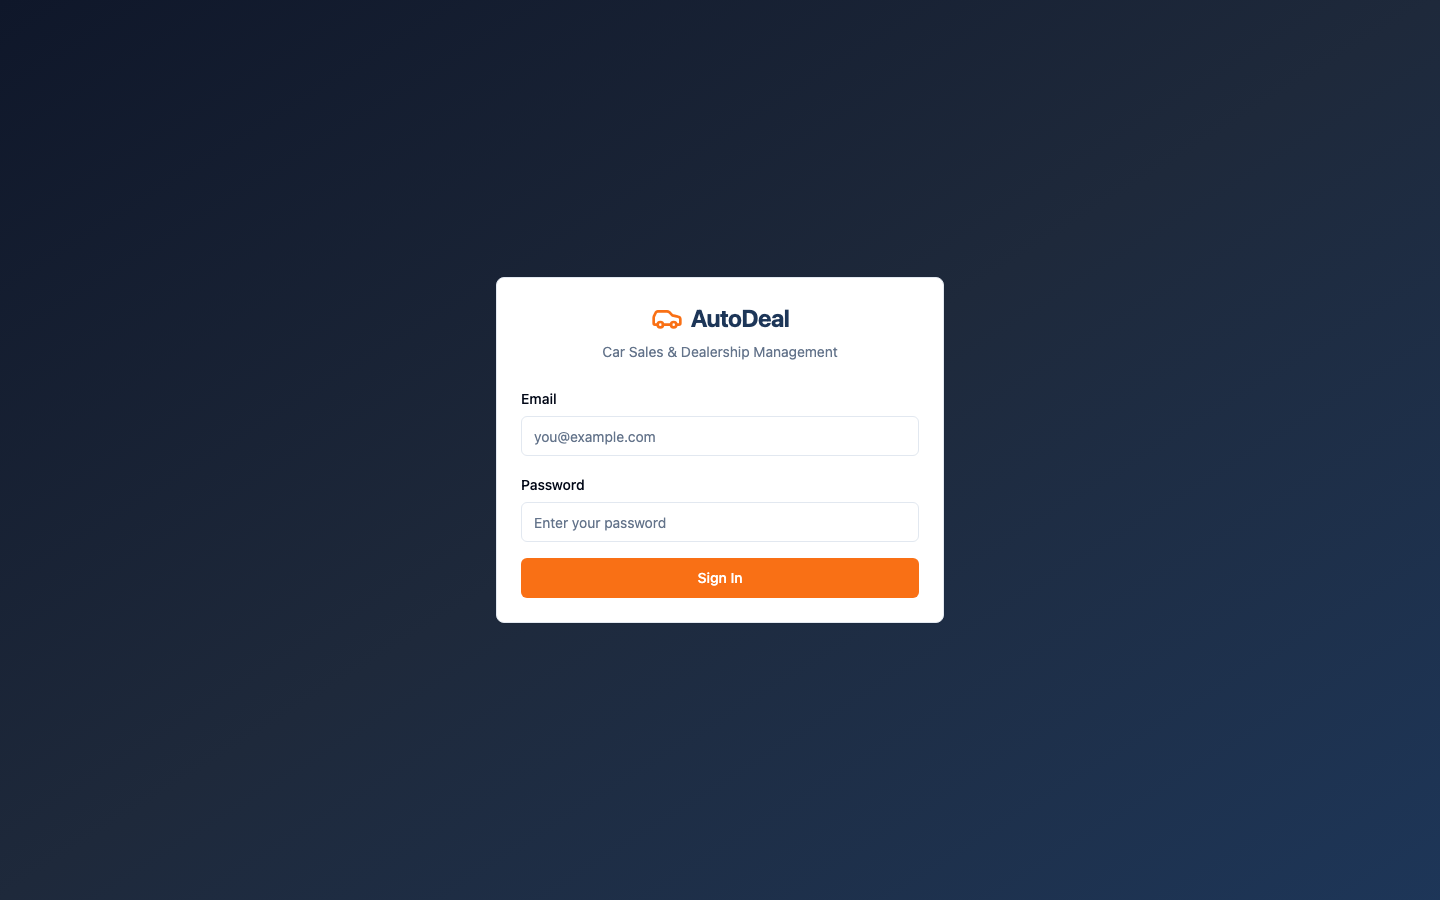
\includegraphics[width=0.85\textwidth]{screenshots/01-login.png}
\caption{Login Page -- Secure authentication with email and password}
\end{figure}

\begin{figure}[H]
\centering
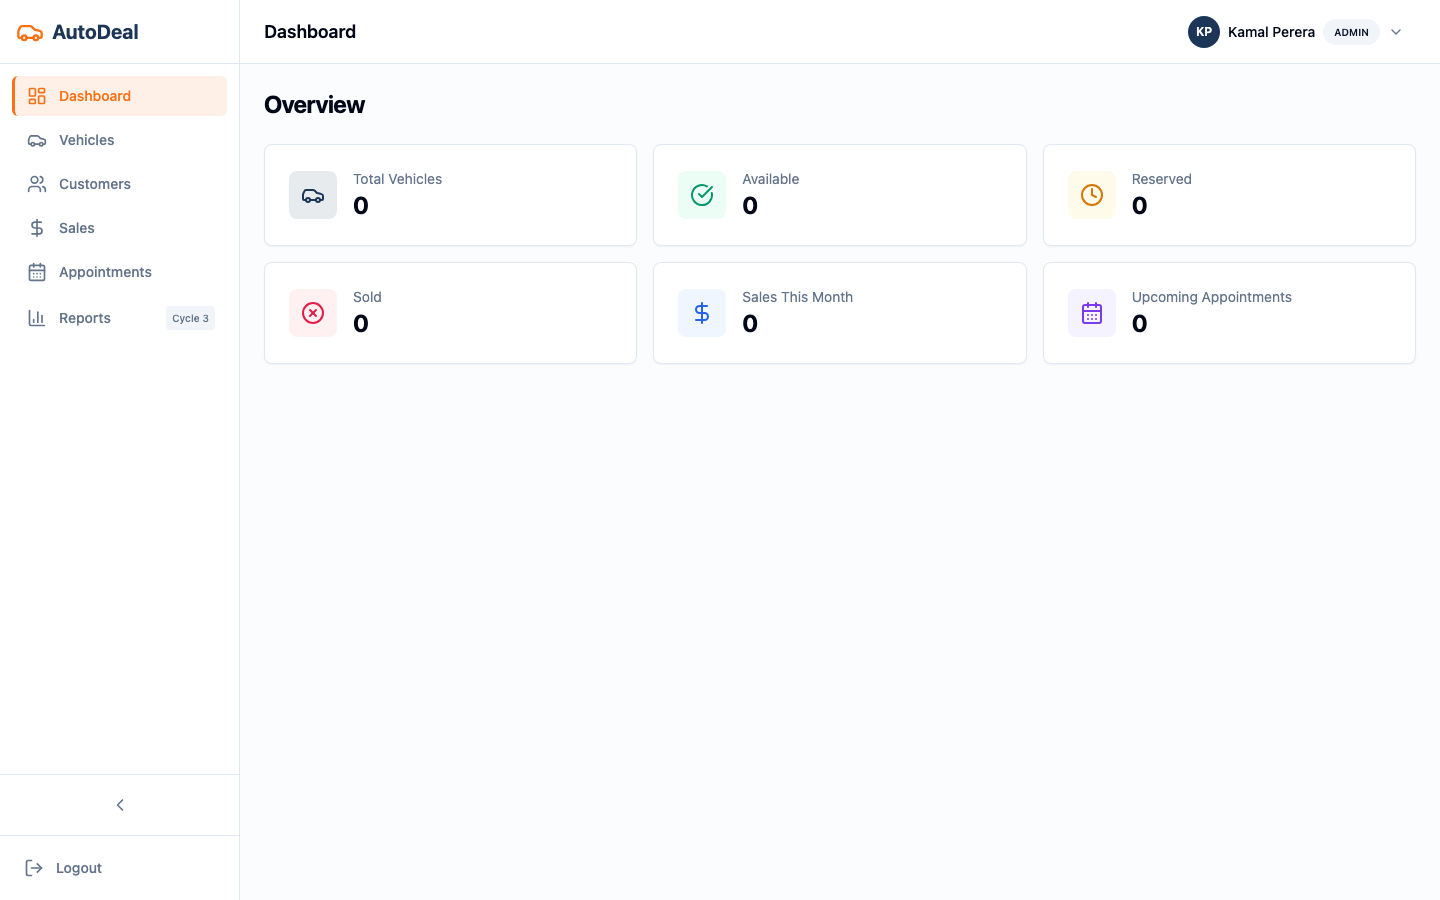
\includegraphics[width=0.95\textwidth]{screenshots/02-dashboard.png}
\caption{Dashboard -- Overview with vehicle, sales, and appointment metrics}
\end{figure}

\begin{figure}[H]
\centering
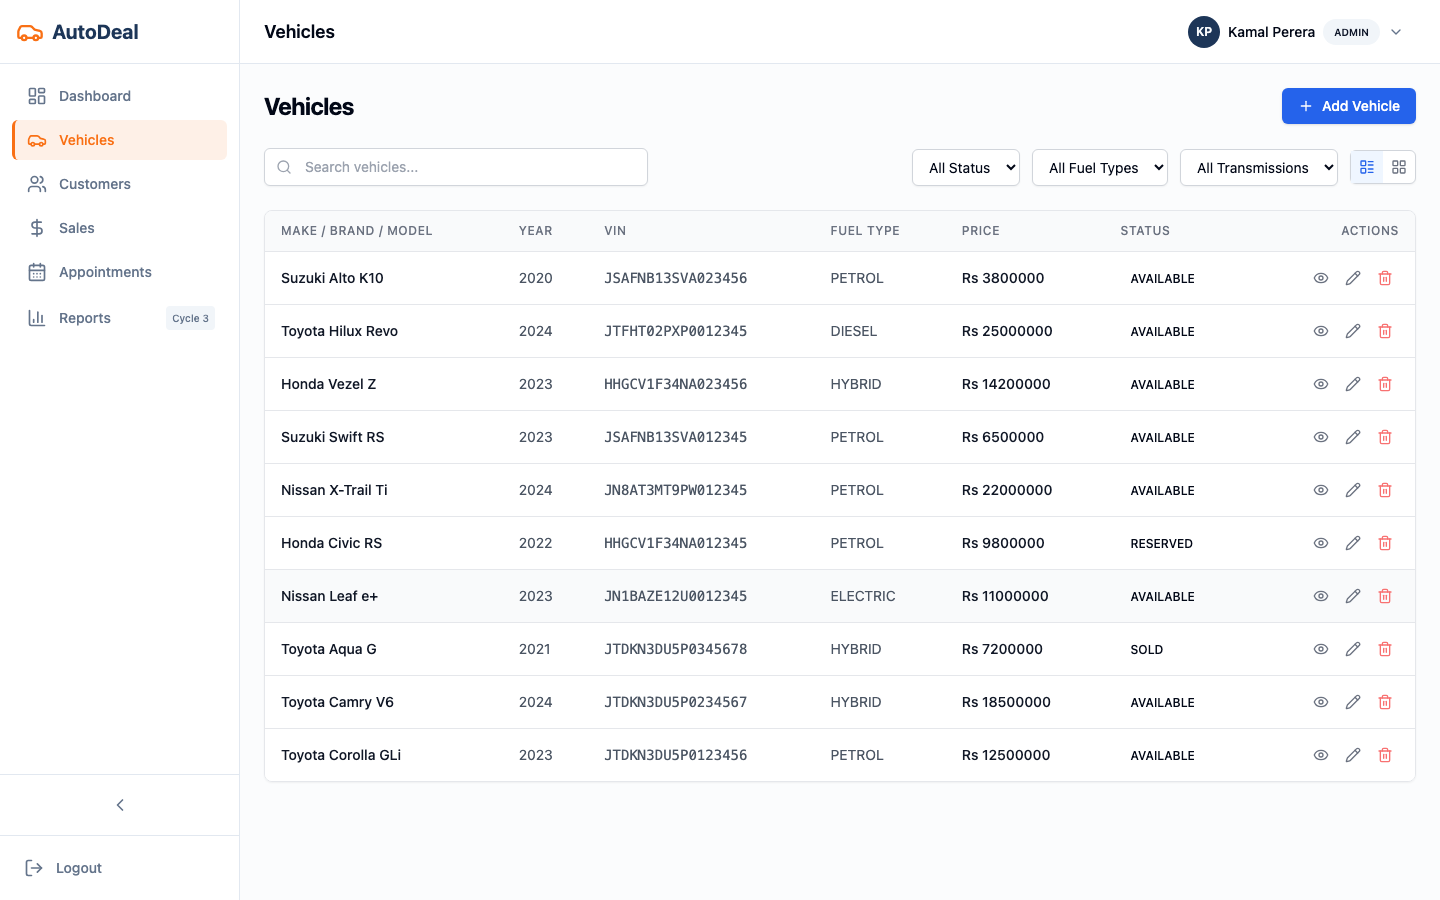
\includegraphics[width=0.95\textwidth]{screenshots/03-vehicles.png}
\caption{Vehicle Inventory -- List view with search, filter, and pagination}
\end{figure}

\begin{figure}[H]
\centering
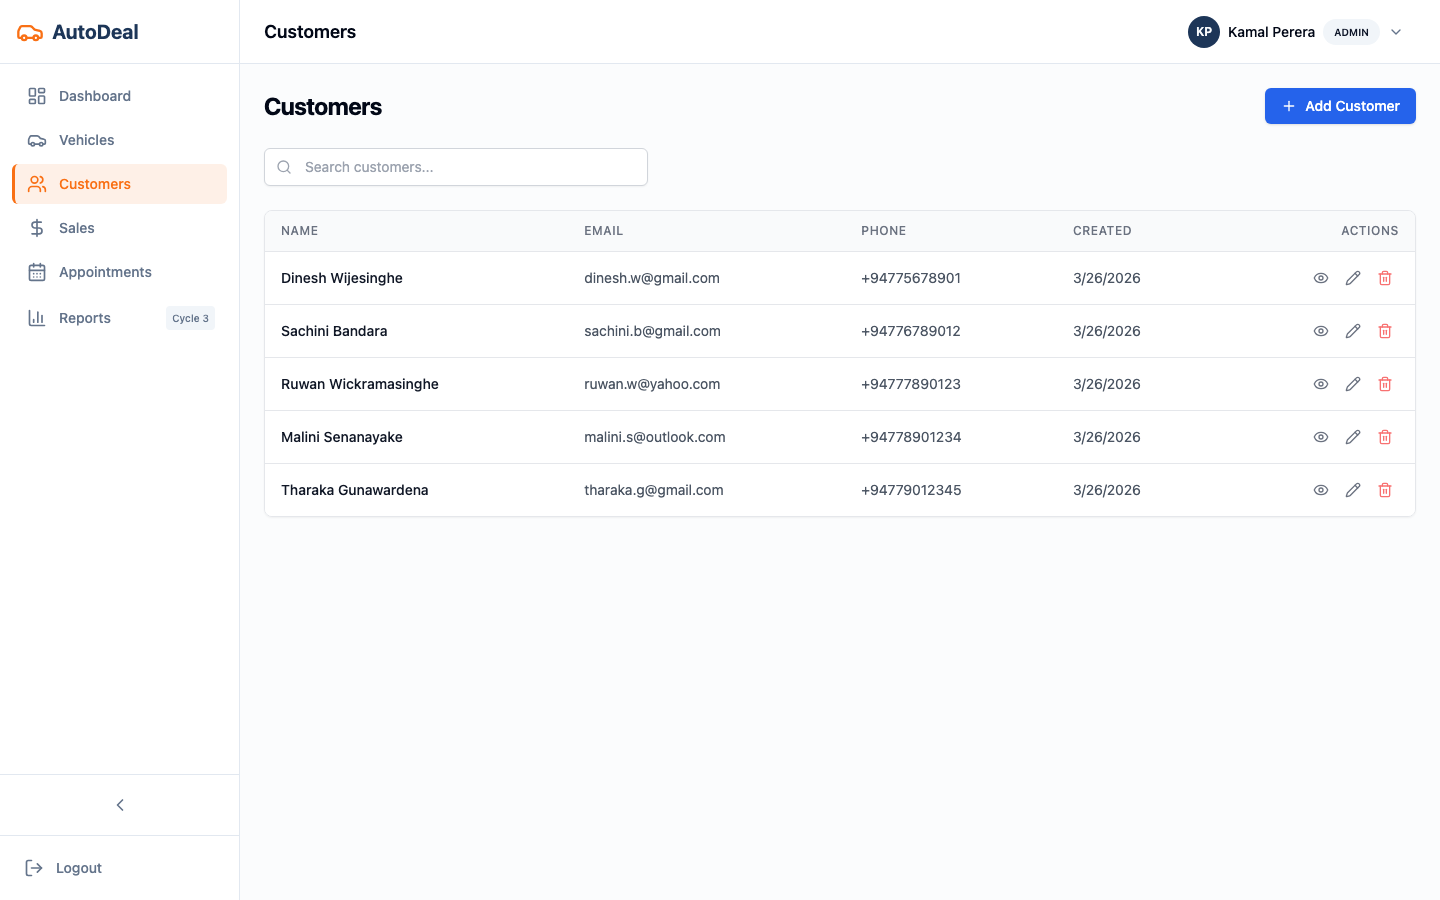
\includegraphics[width=0.95\textwidth]{screenshots/04-customers.png}
\caption{Customer Management -- Customer list with search capabilities}
\end{figure}

\begin{figure}[H]
\centering
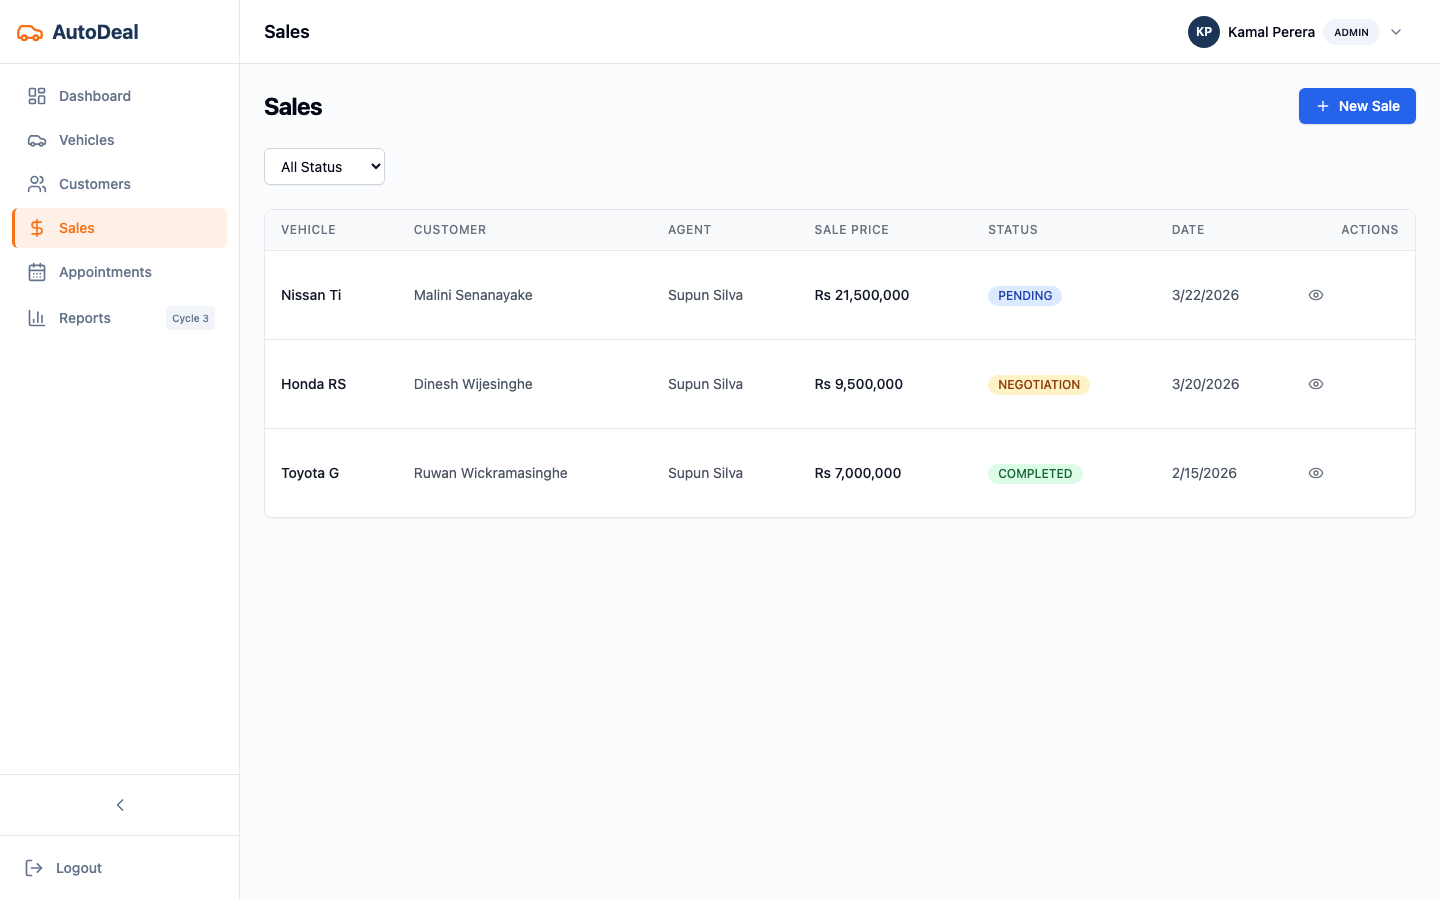
\includegraphics[width=0.95\textwidth]{screenshots/05-sales.png}
\caption{Sales Management -- Sales list with status badges and filtering}
\end{figure}

\begin{figure}[H]
\centering
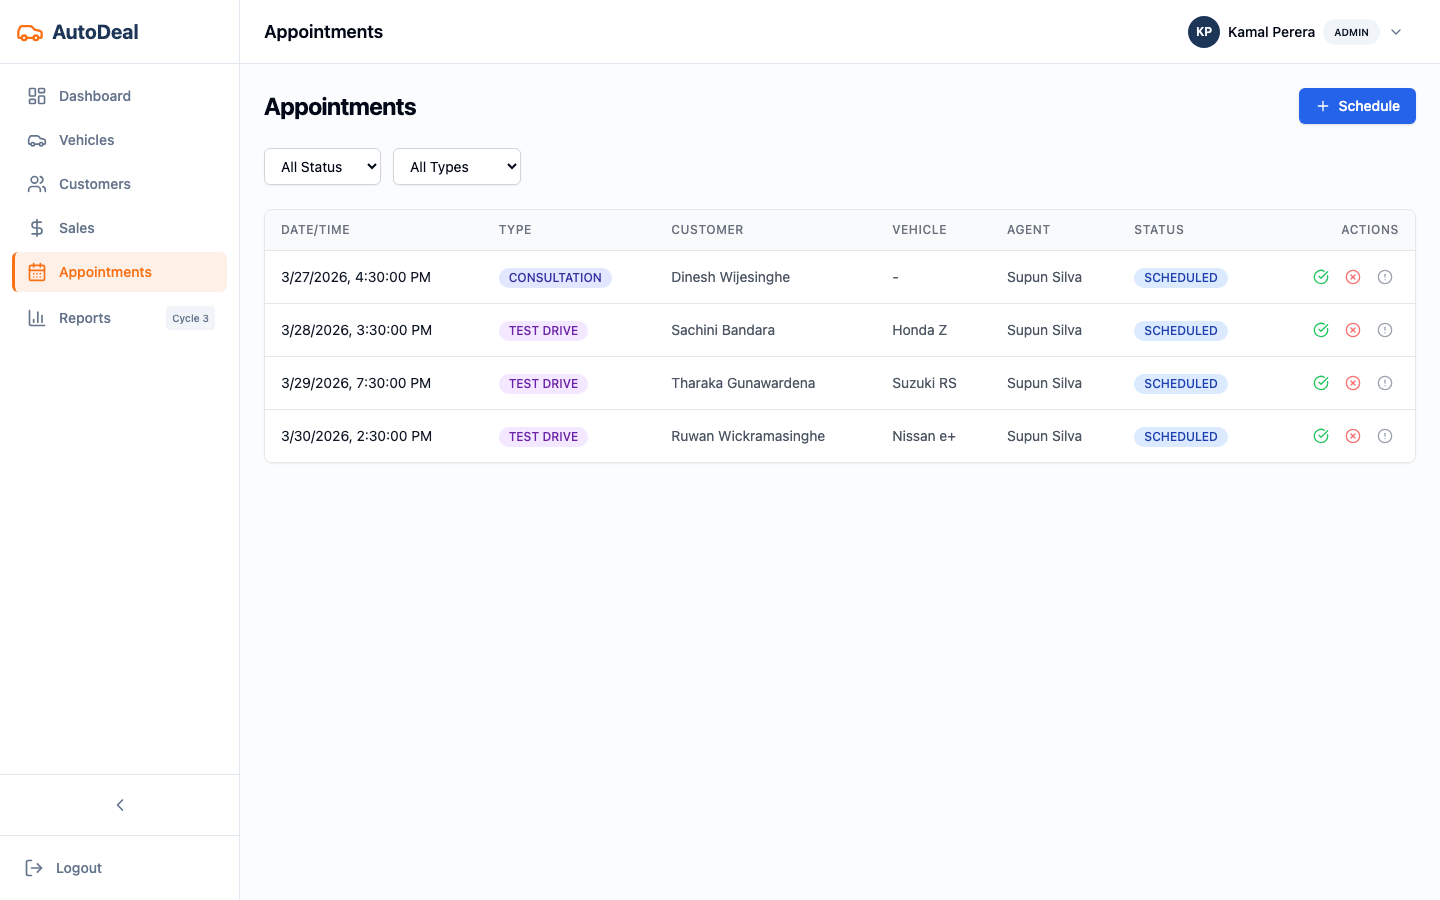
\includegraphics[width=0.95\textwidth]{screenshots/06-appointments.png}
\caption{Appointment Scheduling -- Appointment list with inline status updates}
\end{figure}

\begin{figure}[H]
\centering
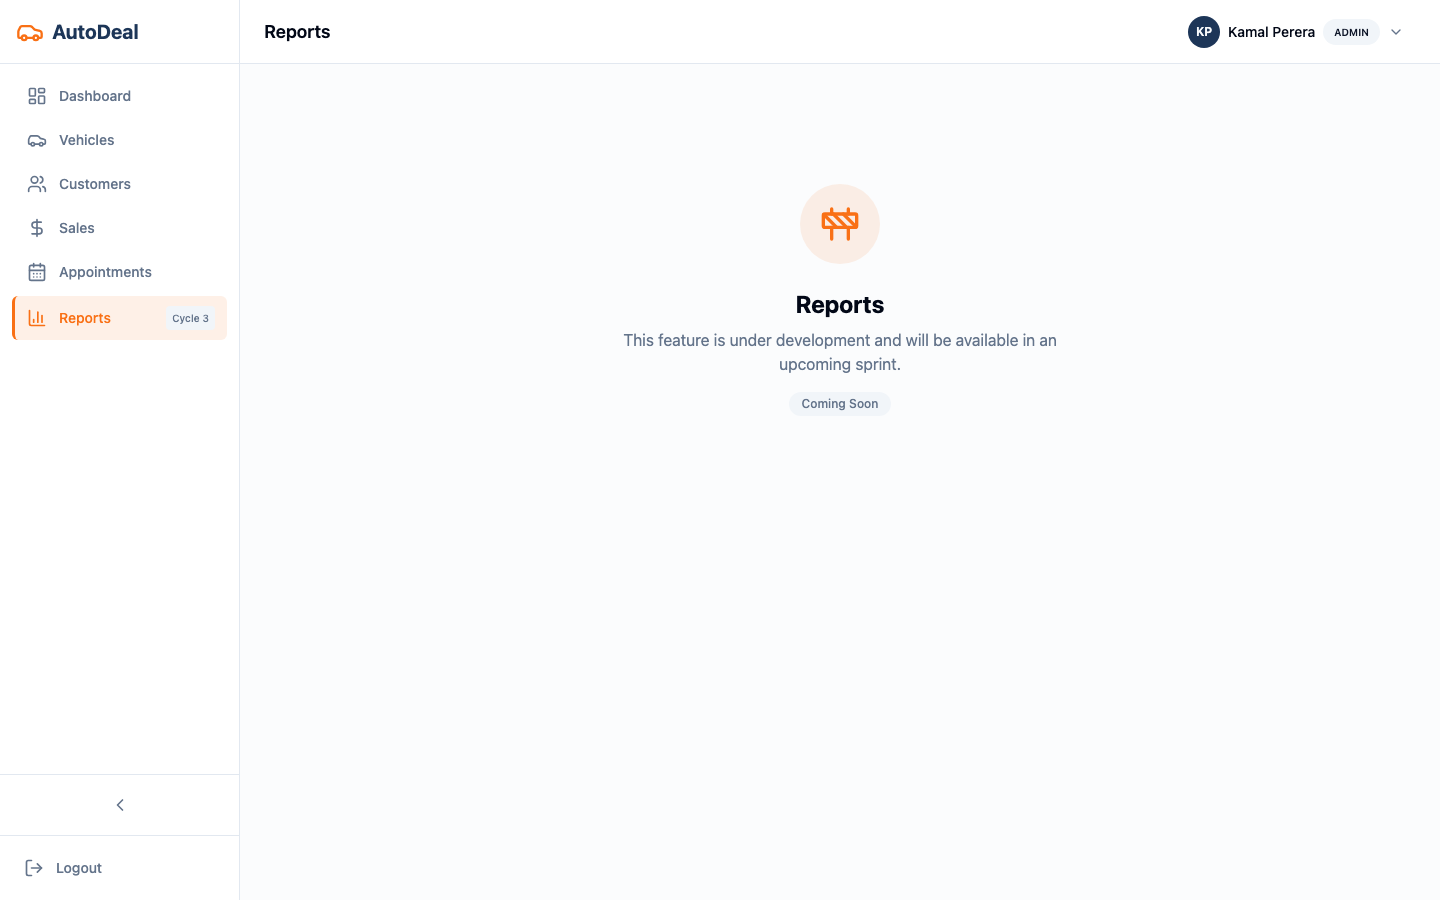
\includegraphics[width=0.95\textwidth]{screenshots/07-coming-soon.png}
\caption{Coming Soon -- Placeholder for features under development}
\end{figure}

% ════════════════════════════════════════════
%  5. TESTING
% ════════════════════════════════════════════
\newpage
\section{Testing Activities and Results}

\subsection{Test Summary}

\begin{table}[H]
\centering
\renewcommand{\arraystretch}{1.3}
\begin{tabularx}{\textwidth}{|l|Y|c|c|c|}
\hline
\rowcolor{HeaderBg} \thead{Module} & \thead{Test Type} & \thead{Total} & \thead{Passed} & \thead{Failed} \\
\hline
Authentication  & Unit & 8 & 8 & 0 \\
\hline
\rowcolor{TableAlt}
Vehicle CRUD    & Unit & 8 & 8 & 0 \\
\hline
Auth Middleware  & Unit & 6 & 6 & 0 \\
\hline
\rowcolor{TableAlt}
Customer CRUD   & Integration & 5 & 5 & 0 \\
\hline
Sales Workflow  & Integration & 6 & 6 & 0 \\
\hline
\rowcolor{TableAlt}
Appointments    & Integration & 4 & 4 & 0 \\
\hline
\textbf{Total}  & & \textbf{37} & \textbf{37} & \textbf{0} \\
\hline
\end{tabularx}
\caption{Sprint 2 Test Results Summary}
\end{table}

\subsection{Key Test Scenarios}

\begin{itemize}[leftmargin=1.5em, itemsep=4pt]
  \item \textbf{Sales -- Complete sale generates invoice:} Creating a sale and transitioning to COMPLETED automatically generates an invoice with correct tax calculation (12\%). \textbf{Result: Passed.}
  \item \textbf{Sales -- Cancel sale reverts vehicle:} Cancelling a NEGOTIATION sale correctly reverts the vehicle status from RESERVED to AVAILABLE. \textbf{Result: Passed.}
  \item \textbf{Appointments -- Double-booking prevention:} Attempting to create overlapping appointments for the same vehicle returns a 409 conflict error. \textbf{Result: Passed.}
  \item \textbf{Customer -- Delete with active sale:} Attempting to delete a customer with a PENDING sale returns a 400 error. \textbf{Result: Passed.}
  \item \textbf{Appointments -- Role-based filtering:} SALES\_AGENT sees only own appointments; ADMIN sees all. \textbf{Result: Passed.}
\end{itemize}

% ════════════════════════════════════════════
%  6. SCRUM ARTIFACTS
% ════════════════════════════════════════════
\section{Scrum Artifacts}

\subsection{Task Board Summary}

\begin{table}[H]
\centering
\renewcommand{\arraystretch}{1.3}
\begin{tabularx}{\textwidth}{|Y|c|c|c|c|}
\hline
\rowcolor{HeaderBg} \thead{Category} & \thead{To Do} & \thead{In Progress} & \thead{In Review} & \thead{Done} \\
\hline
Backend Tasks   & 0 & 0 & 0 & 11 \\
\hline
\rowcolor{TableAlt}
Frontend Tasks  & 0 & 0 & 0 & 10 \\
\hline
Testing/QA      & 0 & 0 & 0 & 4 \\
\hline
\rowcolor{TableAlt}
Documentation   & 0 & 0 & 0 & 3 \\
\hline
DevOps/CI       & 0 & 0 & 0 & 3 \\
\hline
\textbf{Total}  & \textbf{0} & \textbf{0} & \textbf{0} & \textbf{31} \\
\hline
\end{tabularx}
\caption{Sprint 2 Task Board at Sprint End}
\end{table}

\subsection{Burndown}

All 21 planned story points were completed within the sprint. The team achieved a velocity of 21 points, an improvement over Sprint~1's 15 points, reflecting the established development patterns and improved team coordination.

% ════════════════════════════════════════════
%  7. TEAM CONTRIBUTION
% ════════════════════════════════════════════
\needspace{10\baselineskip}
\section{Individual Contributions}

\begin{table}[H]
\centering
\renewcommand{\arraystretch}{1.35}
\footnotesize
\begin{tabularx}{\textwidth}{|l|l|Y|c|}
\hline
\rowcolor{HeaderBg} \thead{Member} & \thead{Role} & \thead{Key Contributions} & \thead{Effort} \\
\hline
P.M.A.D.N.\ Kulathunga & Product Owner & Sprint 2 PRD authoring, acceptance criteria for US05--US08, sales status machine definition, RBAC matrix, Jira backlog management, sprint planning & 22\% \\
\hline
\rowcolor{TableAlt}
B.V.S.M.\ Athurupana & Scrum Master & Daily standup facilitation, Docker deployment configuration with health checks, GitHub Actions CI pipeline, sprint retrospective documentation & 18\% \\
\hline
R.R.M.G.H.\ Rathnayake & Frontend Dev & Customer list/detail/form pages, sales list/detail/create pages, appointment list/create pages, dashboard enhancements, Coming Soon page & 22\% \\
\hline
\rowcolor{TableAlt}
H.M.S.N.\ Rajapaksha & Backend Dev & Customer/Sales/Appointment/Invoice REST APIs, Prisma transaction-based sales workflow, double-booking prevention, auto-invoice generation & 20\% \\
\hline
G.G.P.S.\ Gunathilaka & Full-Stack/QA & Integration testing for sales workflow and appointments, smoke testing customer CRUD, code review, appointment conflict test coverage & 18\% \\
\hline
\end{tabularx}
\caption{Sprint 2 Individual Contributions}
\end{table}

% ════════════════════════════════════════════
%  8. SPRINT REVIEW
% ════════════════════════════════════════════
\section{Sprint Review}

\subsection{Completed Features}

\begin{itemize}[leftmargin=1.5em, itemsep=4pt]
  \item \textbf{Vehicle Edit (Carried from Sprint 1):} Completed the frontend vehicle edit form with full API integration, pre-filled data, and Zod validation -- resolving the Sprint~1 carry-forward item
  \item \textbf{Customer Management:} Full CRUD with search, pagination, and linked sales/appointment history display
  \item \textbf{Sales Workflow:} Complete transaction pipeline with status machine, automatic vehicle status synchronisation, and invoice auto-generation with 12\% VAT
  \item \textbf{Appointment Scheduling:} Test drive and consultation booking with double-booking prevention for both vehicles and agents
  \item \textbf{Invoice System:} Automatic invoice creation on sale completion with amount, tax, and total calculations
  \item \textbf{Dashboard Enhancement:} Six summary cards showing vehicle counts, sales this month, and upcoming appointments
  \item \textbf{Docker Deployment:} Health checks, auto-migration, and seed data on container startup
  \item \textbf{CI Pipeline:} GitHub Actions with TypeScript checking, linting, and test execution
\end{itemize}

\subsection{Incomplete / Carried Forward}

\begin{itemize}[leftmargin=1.5em, itemsep=4pt]
  \item No items carried forward. All Sprint 2 user stories were completed successfully.
\end{itemize}

% ════════════════════════════════════════════
%  9. SPRINT RETROSPECTIVE
% ════════════════════════════════════════════
\needspace{10\baselineskip}
\section{Sprint Retrospective}

\subsection{What Went Well}

\begin{itemize}[leftmargin=1.5em, itemsep=4pt]
  \item Established development patterns from Sprint 1 significantly accelerated Sprint 2 development. The service-route-validator module structure enabled rapid feature addition.
  \item Prisma transactions ensured data consistency across the complex sales workflow involving vehicle status updates and invoice generation.
  \item Docker containerisation allowed all team members to develop against identical environments, eliminating ``works on my machine'' issues.
\end{itemize}

\subsection{What Could Be Improved}

\begin{itemize}[leftmargin=1.5em, itemsep=4pt]
  \item Frontend test coverage remains lower than backend. Sprint 3 should prioritise React Testing Library tests for critical user flows.
  \item The appointment scheduling UI would benefit from a calendar view rather than a simple list to better visualise scheduling conflicts.
\end{itemize}

\subsection{Action Items for Sprint 3}

\begin{table}[H]
\centering
\renewcommand{\arraystretch}{1.3}
\begin{tabularx}{\textwidth}{|c|Y|l|}
\hline
\rowcolor{HeaderBg} \thead{\#} & \thead{Action Item} & \thead{Owner} \\
\hline
1 & Implement analytics dashboard with recharts for sales performance and inventory trends & Frontend Dev \\
\hline
\rowcolor{TableAlt}
2 & Build invoice PDF generation and inventory reporting endpoints & Backend Dev \\
\hline
3 & Increase frontend test coverage to $\geq$60\% with React Testing Library & Full-Stack/QA \\
\hline
\end{tabularx}
\caption{Retrospective Action Items}
\end{table}

% ════════════════════════════════════════════
%  10. SPRINT 3 PLAN
% ════════════════════════════════════════════
\needspace{8\baselineskip}
\section{Sprint 3 Preview}

\subsection{Sprint 3 Goal}

Implement analytics dashboard with visual charts, sales agent performance tracking, invoice generation for completed sales, and inventory reporting.

\subsection{Planned User Stories}

\begin{table}[H]
\centering
\renewcommand{\arraystretch}{1.3}
\footnotesize
\begin{tabularx}{\textwidth}{|c|Y|c|c|}
\hline
\rowcolor{HeaderBg} \thead{ID} & \thead{User Story} & \thead{Priority} & \thead{Points} \\
\hline
\textbf{US09} & As a manager, I want to view a sales analytics dashboard so that I can monitor dealership performance & Should & 8 \\
\hline
\rowcolor{TableAlt}
\textbf{US10} & As a manager, I want to track sales agent performance and commissions so that I can manage the sales team effectively & Should & 5 \\
\hline
\textbf{US11} & As a sales agent, I want to generate invoices for completed sales so that customers receive proper documentation & Should & 5 \\
\hline
\rowcolor{TableAlt}
\textbf{US12} & As a manager, I want to view inventory reports showing stock levels and turnover rates & Should & 5 \\
\hline
\end{tabularx}
\caption{Sprint 3 Planned Backlog}
\end{table}


\end{document}
